\section{Auswertung}
Zur qualtitativen Diskussion der Messergebnisse sollen im folgenden Abschnitt relevante Rechnungen mit den gefundenen
Werten durchgeführt werden. Fehlerfortpflanzungen, sowie Ausgleichsrechnungen werden mit
Hilfe der Python Bibliotheken \emph{uncertainties}\cite{uncertainties} und \emph{scipy}\cite{scipy} bestimmt.
\subsection{1}
Die Messwerte zur Untersuchung des zeitlichen Verlaufs der Kondensatorspannungsamplitude $A(t)$ sind in Tabelle \ref{tab: amplitude} aufgetragen. Wie in der Theorie erwähnt,
lässt sich der Verlauf durch eine Funktion der Form
\begin{equation}
  A(t) = A_0 \, \exp[-B\cdot t]
\end{equation}
darstellen. Für die Parameter ergeben sich die Werte:
\begin{align}
  B &= \SI{4907.68(26870)}{\second^{-1}}\\
  A_0 &= \SI{5.16(13)}{\volt}.
\end{align}
Die Fit-Funktion, sowie die Messwerte sind in Abbildung \ref{fig: amplitude} dargestellt.
Mit dem Parameter $B$ lässt sich der effektive Widerstand $R\ua{eff}$ bestimmen.
\begin{equation}
  B = \frac{R\ua{eff}}{2L} \quad \Rightarrow \quad R\ua{eff} =  \SI{99(5)}{\ohm}.
  \label{eq: Fitparameter}
\end{equation}
Des Weiteren ergibt sich aus der Ausgleichsrechnenung für die Abklingzeit $T\ua{ex}$:
\begin{equation}
  B = \frac{1}{T\ua{ex}} \quad \Rightarrow \quad T\ua{ex} =  \SI{2.04(11)e-4}{\second}.
\end{equation}
Mittels der Gleichung \eqref{} kann der entsprechende Theoriewert, sowie die prozentuale Abweichung bestimmt werden:
\begin{align}
  \begin{aligned}
  T\ua{ex, th} &= \SI{4.21e-4}{\second}\\
  d_{T\ua{ex}} &= \SI{-52}{\percent}.
\end{aligned}
\label{eq: theo_breite}
\end{align}
Der gefundenen Wert für den
Widerstand der Schaltung weicht um etwa $\SI{51}{\ohm}$ von dem verbauten Widerstand ($R =  \SI{48}{\ohm}$) ab. Dies kann
auf nicht betrachtete Innenwiderstände des Generators bzw. anderer Bauteile zurückgeführt werden und stellt
gleichzeitig eine Erklärung für die deutliche prozentuale Abweichung der charakteristischen Abklingzeit vom Theoriewert dar.
\begin{table} 
\centering 
\caption{Zeitlicher Verlauf der Amplitude des gedämpften Schwingkreises} 
\label{tab: amplitude} 
\begin{tabular}{S S } 
\toprule  
{$t$ / $10^{-5}\si{\second}$} & {$A$ / $\si{\volt}$}  \\ 
\midrule  
 0.0  & 9.84\\ 
3.0  & 9.04\\ 
6.0  & 8.40\\ 
9.0  & 7.92\\ 
12.0  & 7.52\\ 
15.0  & 7.12\\ 
18.0  & 6.80\\ 
21.0  & 6.56\\ 
24.0  & 6.16\\ 
27.0  & 5.92\\ 
30.0  & 5.76\\ 
33.0  & 5.68\\ 
36.0  & 5.52\\ 
\bottomrule 
\end{tabular} 
\end{table}
\begin{figure}
  \centering
  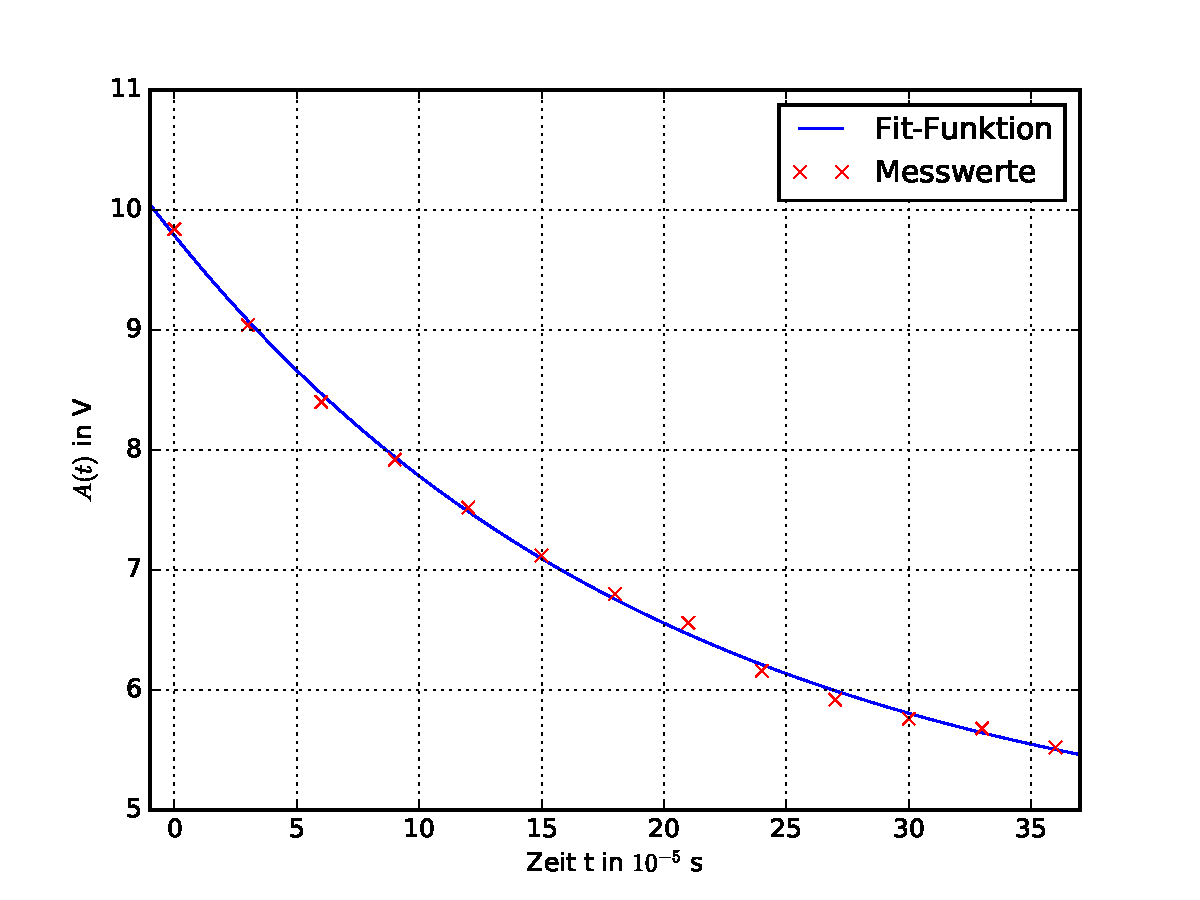
\includegraphics[width = \textwidth]{../Messdaten/amplitude.pdf}
  \caption{Zeitlicher Verlauf der Kondensatorspannungsamplitude des gedämpften Schwingkreises und Fit-Funktion.}
  \label{fig: amplitude}
\end{figure}

\subsection{Frequenzabhängigkeit der Kondensatorspannung}
Die gemessenen Werte der Generator- und Kondensatorspannung unter variabler Frequenz sind in Tabelle \ref{tab: frequenzabhängigkeit} aufgeführt.
Hierbei ist zu erkennen, dass bei den ersten neun Messwerten, die in kleinen Frequnezbereichen aufgenommen wurden, nur eine geringfügige
Diskrepanz zwischen beiden Größen besteht. Die graphische Darstellung der Werte bei höheren Frequenzen ist in Abbildung \ref{fig: spannungsverlauf_U_C}
einzusehen. Für die Resonanzfrequenz entnimmt man aus der Messreihe den Wert:
\begin{equation}
  \nu_{0, exp} = \SI{33}{\kilo\hertz}.
  \label{eq: exp_resonanzfrequenz}
\end{equation}
Gemäß Formel \eqref{eq:resonanzfrequenz} berechnet sich der Theoriewert der Resonanzfrequenz $\nu_{0, th}$, sowie die prozentuale Abweichung $d_{\nu}$ des gemessenen Wertes zu:
\begin{align}
  \begin{aligned}
  \nu_{0, th} &= \SI{3.409e4}{\hertz} \\
  d_{\nu} &= \SI{-3.19}{\percent}.
\end{aligned}
\label{eq: theo_resonanzfrequenz}
\end{align}
Des Weiteren entnimmt man aus der graphischen Darstellung die Größen $\nu_+$ und $\nu_-$, aus denen die Breite der Resonanzkurve bestimmt werden kann.
\begin{align}
  \begin{aligned}
  \nu_{+} &= \SI{3.745e4}{\hertz} \\
  \nu_{-} &= \SI{2.860e4}{\hertz} \\
  (\nu_{+}-\nu_{-})_{exp} &= \SI{8.85e3}{\hertz}.
\end{aligned}
\label{eq: breite_exp}
\end{align}
Für den Theoriewert der Breite [gemäß \eqref{eq:omega_+_-}] und die prozentuale Abweichung ergeben sich hieraus:
\begin{align}
  \begin{aligned}
  (\nu_{+}-\nu_{-})_{th} &= \SI{8.02e3}{\hertz}\\
  d_{\nu_{+}-\nu_{-}} &= \SI{10.34}{\percent}.
\end{aligned}
\label{eq: theo_breite}
\end{align}
\begin{figure}
  \centering
  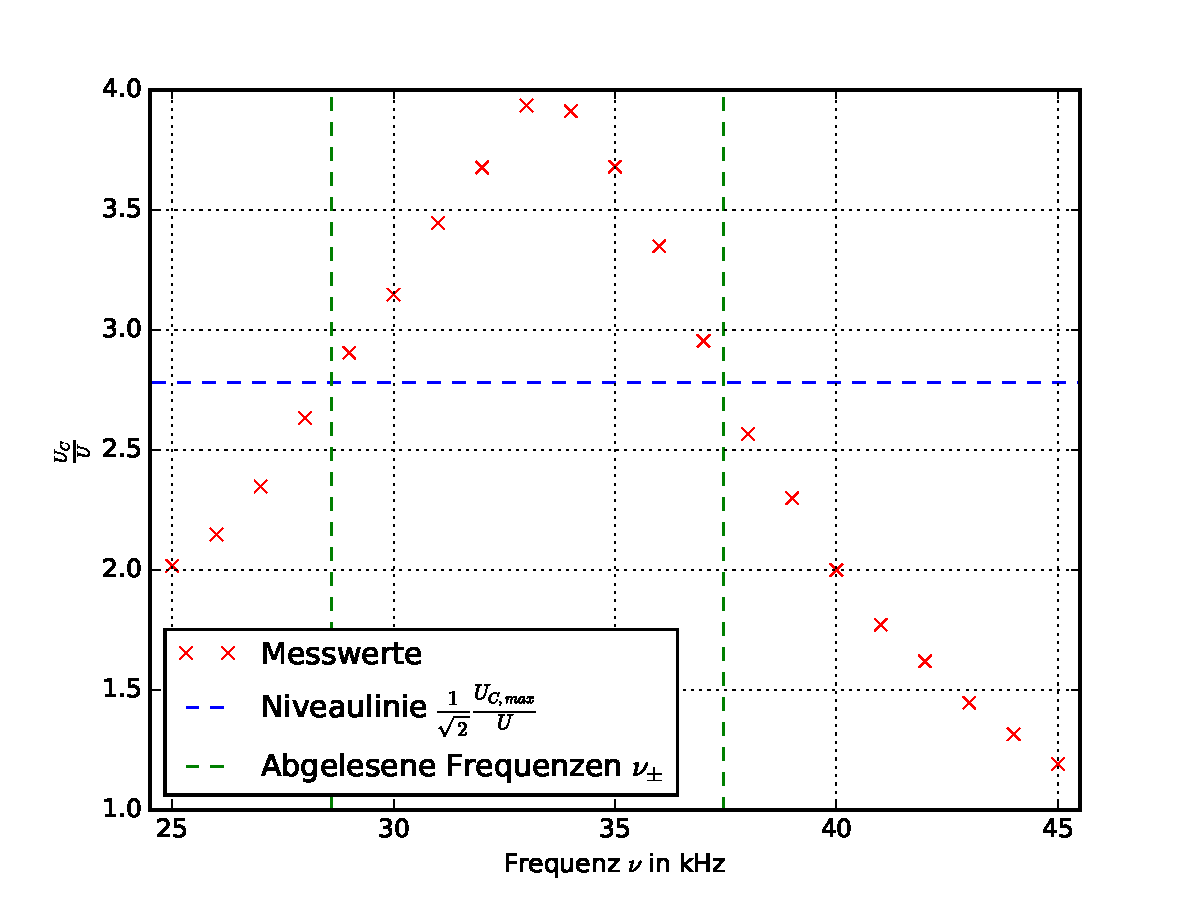
\includegraphics[width = \textwidth]{../Messdaten/U_f_linear.pdf}
  \caption{Verlauf der normierten Spannung am Kondensator unter variabler Frequenz, sowie eingezeichnete Hilfslinien zum Ablesen der relevanten Größen.}
  \label{fig: spannungsverlauf_U_C}
\end{figure}
Die Resonanzüberhöhung berechnet sich theoretisch gemäß Formel \eqref{eq: resonanzüberhöhung} zu:
\begin{equation}
  q\ua{th} = \SI{4.25}.
\end{equation}
Aus der Messung gewinnt man den entsprechenden experimentellen Wert:
\begin{equation}
    q\ua{exp} = \SI{3.94}.
\end{equation}
Der gefundene Wert weicht somit um
\begin{equation}
  d\ua{q} = \SI{7}{\percent}
\end{equation}
vom theoretischen Wert ab.

\subsection{Frequenzabhängigkeit der Phasenverschiebung}
Die mit dem Oszilloskop bestimmten Werte für die Phasenlänge der Generatorspannung $b$ und den zeitlichen Versatz $a$ zur Kondensatorspannung, sowie die gemäß \eqref{eq:phasen_unterschied}
errechnete Phasenverschiebung $\varphi$ sind ebenfalls in Tabelle \ref{tab: frequenzabhängigkeit} aufgetragen. Auch hier zeigt sich bei den niedrigen
Frequenzen kein signifikanter Effekt. Eine graphische Darstellung der Werte bei hohen Frequenzen befindet sich in
Abbildung \ref{fig: phasenverlauf}. Aus der Abbildung bzw. den Daten entnimmt man für den Wert, bei dem die Phasendifferenz $\frac{\pi}{2}$ beträgt:
\begin{equation}
  \nu_0 = \SI{34}{\kilo\hertz}
\end{equation}
Dieser zweite experimentell bestimmte Wert für die Resonanzfrequenz weicht um
\begin{equation}
  d_{\nu} = \SI{-0.26}{\percent}
\end{equation}
von dem in \eqref{eq: theo_resonanzfrequenz} berechneten Theoriewert ab.
Weiter werden als Werte für $\nu_+$ und $\nu_-$ jene Frequenzen abgelesen, bei denen die Phasenverschiebung
gerade $\frac{3\pi}{4}$ bzw. $\frac{\pi}{4}$ beträgt. Hieraus kann erneut die Breite und die Abweichung
zum Theoriewert \eqref{eq: theo_breite} bestimmt werden:
\begin{align}
  \begin{aligned}
  \nu_{+} &= \SI{30.0}{\kilo\hertz} \\
  \nu_{-} &= \SI{36.5}{\kilo\hertz} \\
  (\nu_{+}-\nu_{-})_{exp} &= \SI{6.5e3}{\hertz} \\
  d_{\nu_{+}-\nu_{-}} &= \SI{-18.96}{\percent}.
\end{aligned}
\end{align}
\begin{table} 
\centering 
\caption{Messwerte der Zeitparameter a und b, Kondensator- und Generatorspannung, sowie die errechnete Phasendifferenz in Abhängigkeit von der Frequenz $\nu$.} 
\label{tab: frequenzabhängigkeit} 
\begin{tabular}{S S S S S S } 
\toprule  
{$\nu$ / \si{\hertz}} & {$U$ / $\si{\volt}$} & {$U_C$ / $\si{\volt}$} & {$a$ / $\si{\micro\second}$} & {$b$ / $\si{\micro\second}$} & {$\phi$ / rad}  \\ 
\midrule  
 10  & 4.64  & 4.64  & 0.00  & 100000.00  & 0.00\\ 
25  & 4.64  & 4.64  & 0.00  & 40000.00  & 0.00\\ 
500  & 4.64  & 4.60  & 0.00  & 2000.00  & 0.00\\ 
1000  & 4.64  & 4.64  & 0.00  & 1000.00  & 0.00\\ 
5000  & 4.68  & 4.80  & 0.00  & 200.00  & 0.00\\ 
5500  & 4.72  & 4.84  & 0.00  & 180.00  & 0.00\\ 
6000  & 4.80  & 4.84  & 1.10  & 167.00  & 0.04\\ 
6500  & 4.80  & 4.88  & 1.10  & 153.00  & 0.05\\ 
7000  & 4.72  & 4.92  & 1.20  & 142.00  & 0.05\\ 
25000  & 4.56  & 9.20  & 3.16  & 40.00  & 0.50\\ 
26000  & 4.60  & 9.88  & 3.44  & 38.48  & 0.56\\ 
27000  & 4.60  & 10.80  & 3.76  & 36.92  & 0.64\\ 
28000  & 4.48  & 11.80  & 4.18  & 35.75  & 0.73\\ 
29000  & 4.44  & 12.90  & 3.56  & 34.48  & 0.65\\ 
30000  & 4.48  & 14.10  & 4.06  & 33.30  & 0.77\\ 
31000  & 4.44  & 15.30  & 6.71  & 32.20  & 1.31\\ 
32000  & 4.46  & 16.40  & 6.71  & 31.26  & 1.35\\ 
33000  & 4.32  & 17.00  & 6.40  & 30.27  & 1.33\\ 
34000  & 4.32  & 16.90  & 7.36  & 29.46  & 1.57\\ 
35000  & 4.32  & 15.90  & 9.32  & 28.50  & 2.05\\ 
36000  & 4.36  & 14.60  & 9.80  & 27.85  & 2.21\\ 
37000  & 4.40  & 13.00  & 10.30  & 26.95  & 2.40\\ 
38000  & 4.48  & 11.50  & 10.50  & 26.32  & 2.51\\ 
39000  & 4.48  & 10.30  & 9.72  & 25.64  & 2.38\\ 
40000  & 4.52  & 9.04  & 9.80  & 24.92  & 2.47\\ 
41000  & 4.56  & 8.08  & 10.40  & 24.38  & 2.68\\ 
42000  & 4.52  & 7.32  & 10.30  & 23.92  & 2.71\\ 
43000  & 4.56  & 6.60  & 9.70  & 23.24  & 2.62\\ 
44000  & 4.56  & 6.00  & 9.40  & 22.74  & 2.60\\ 
45000  & 4.60  & 5.48  & 9.60  & 22.27  & 2.71\\ 
\bottomrule 
\end{tabular} 
\end{table}

\begin{figure}
  \centering
  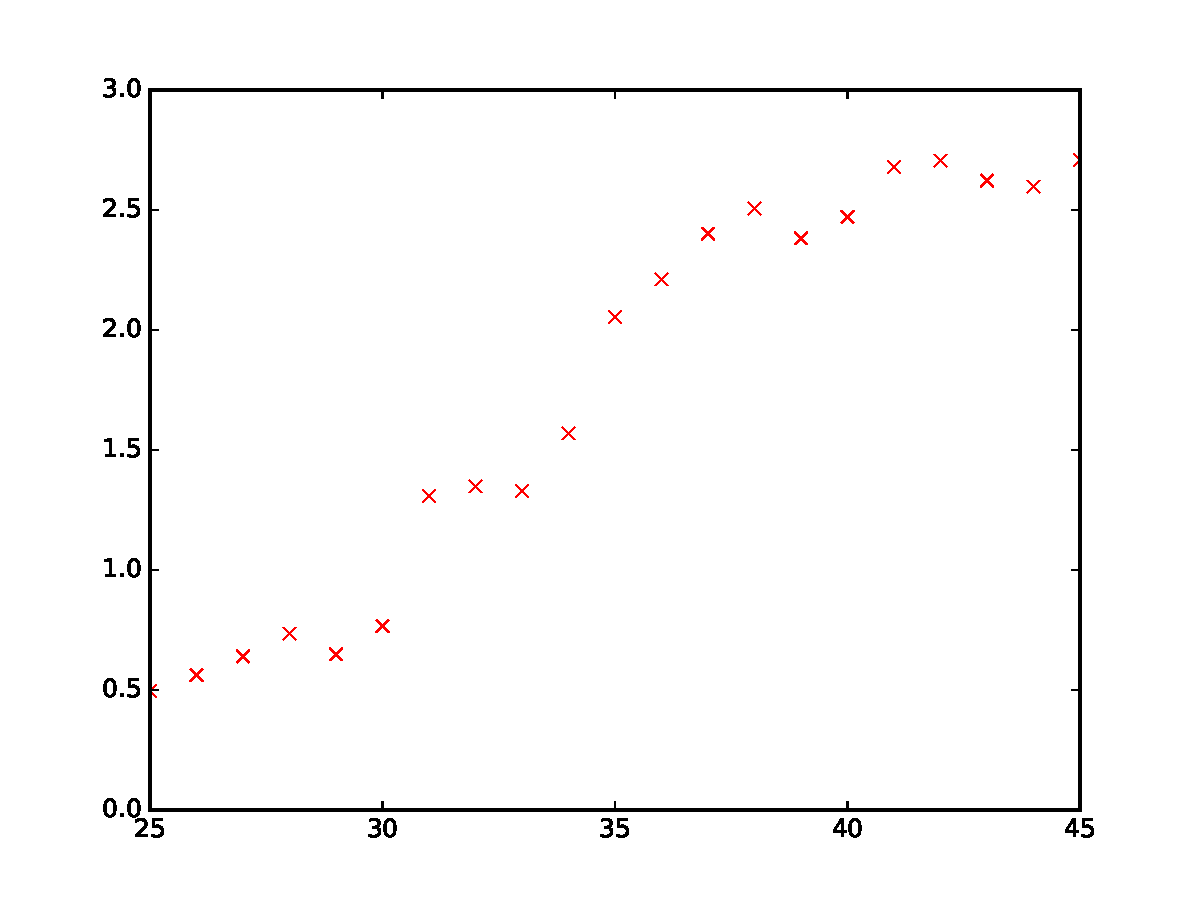
\includegraphics[width = \textwidth]{../Messdaten/phase_f_linear.pdf}
  \caption{Verlauf der Phasendifferenz zwischen Erreger- und Kondensatorspannung unter variabler Frequenz.}
  \label{fig: phasenverlauf}
\end{figure}


\subsection{Bestimmung des Widerstandes $R\ua{AP}$}
Aus der Messung wurde folgender Wert für den Widerstand $R\ua{AP}$ gewonnen:
\begin{equation}
  R\ua{AP, exp} = \SI{28.0}{\kilo\ohm}.
\end{equation}
Mit Formel \eqref{} erhält man den theoretischen Wert:
\begin{equation}
    R\ua{AP, th} = \SI{4.4}{\kilo\ohm}.
\end{equation}
Als prozentuale Abweichung zwischen theoretischem und experimentellem Ergebnis berechnet sich:
\begin{equation}
  d\ua{R\ua{AP}} = \SI{538}{\percent}
\end{equation}
Diese große Abweichung lässt sich durch die ungenaue Messung des Widerstandes erklären. Einerseits kann der gesuchte Punkt,
an dem es zu keinen Überschwingern mehr kommt, nur sehr schwer erkannt werden. Darüber hinaus stellt die Skala, an der der Widerstand
letztendlich abgelesen wurde eine Quelle für systematische Fehler dar.
